\documentclass[a4paper]{article}
\usepackage{a4wide}
\usepackage{amsmath}
\usepackage{amsfonts}
  \DeclareMathOperator*{\argmax}{arg\,max}
  \newcommand{\ex}[1]{{\mathbb E}\left[ #1 \right]}
  \newcommand\norm[1]{\left\lVert#1\right\rVert}
\usepackage{booktabs}
\usepackage{csquotes}
\usepackage{upquote}
\usepackage{float}
\usepackage{graphicx}
\usepackage{enumerate}
\usepackage{subcaption}
\usepackage[most]{tcolorbox}
\usepackage{xcolor}
\usepackage{varwidth} 


\title{Pattern and Speech Recognition WS2015-16 \\ Exercise 7}
\author{Atanas Poibrenski(2554135), Marimuthu Kalimuthu(2557695), Furkat Kochkarov(2557017)}

\begin{document}
	\tcbset{
		enhanced,
		colback=red!5!white,
		boxrule=0.1pt,
		colframe=red!75!black,
		fonttitle=\bfseries
	}

\maketitle 
\begin{center}
	\textbf{Decision Trees}
\end{center}

\section*{Exercise 1}
\begin{enumerate}
	\item[ \textbf{1} ] Done.
	\item[ \textbf{2} ] See ``decision\_tree.m"
	\item[ \textbf{3} ] Histogram plot:
	\begin{figure}[H]
		\begin{center}
			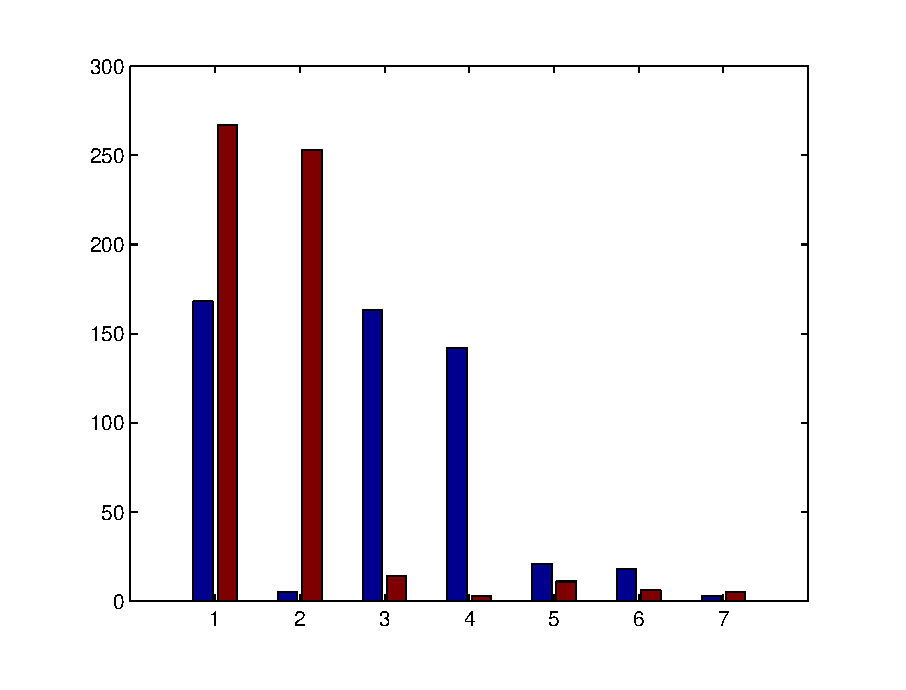
\includegraphics[width=1.0\textwidth]{hists.eps}
			\caption{Histogram for two class labels (blue=republican, red=democrat) }\label{fig:hist_1.3}
		\end{center}
	\end{figure}
	
	(From the histogram), the highest probability class at every node are as follows:
	
	\begin{tcolorbox}
	\begin{align*}
		& node1 = democrat  \\
		& node2 = democrat   \\
		& node3 = republican  \\
		& node4 = republican  \\
		& node5 = republican \\
		& node6 = republican \\
		& node7 = democrat		
	\end{align*}
	\end{tcolorbox}
			
	The histogram tells us that the quality of the questions is good since the splits result in low misclassification rates and are almost pure.
	
	\item[ \textbf{4} ] Misclassification Rates:
	    \begin{tcolorbox}
		\begin{align*}
			& node1 = 0.38 \\
			& node2 = 0.019 \\
			& node3 = 0.07  \\
			& node4 = 0.02  \\
			& node5 = 0.34  \\
			& node6 = 0.25  \\
			& node7 = 0.375
		\end{align*}
    \end{tcolorbox}
    
	\item[ \textbf{5} ] Entropy of the nodes:
	%ex 1.5 entropy of each node
		\begin{tcolorbox}
		\begin{align*}
			& node1 = 0.96  \\
			& node2 = 0.137  \\
			& node3 = 0.398  \\
			& node4 = 0.145  \\
			& node5 = 0.92  \\
			& node6 = 0.811  \\
			& node7 = 0.95
		\end{align*}
	\end{tcolorbox}
	
	\item[ \textbf{6} ] Information Gain:
	    \begin{tcolorbox}
	    \begin{align*}
		  %ex 1.6 information gain of non-leaf nodes
		  & node1 = 0.96 - (258/435 * 0.137 + 167/435 * 0.398)
		          = 0.72  \\ 
		  & node2 = 0.398 - (145/177 * 0.145 + 32/177 * 0.92)
		          = 0.11  \\
		  & node3 = 0.92 - (24/32 * 0.811 + 8/32 * 0.95)
		          = 0.07  \\
	    \end{align*}
	    \end{tcolorbox}
	
	\item[ \textbf{7} ] Why Information Gain? \newline
	The information gain is a good measure because for a given node, maximizing the information gain is equivalent to minimizing the entropy of its children. Minimizing the entropy of the children will result in more ``purity", therefore less classification error. \newline \newline
	The question about \textit{anti-satellite-test-ban} will maximize the information gain. This question will result in \textit{pure splits}.
	
	\item[ \textbf{8} ] Algorithm to construct complete decision tree: \newline
	* Start with the \textit{root node}. \newline
	* For all the possible questions to ask, choose the one which results into the highest possible information gain. \newline
	* Repeat this for all the nodes. \newline
	* If a splitting of a node results into a \textit{pure split}, stop splitting on that node.
	
\end{enumerate}

\section*{Exercise-2}
	\begin{enumerate}
		\item[ \textbf{1} ] Prior probabilities of the classes:
		
		\begin{tcolorbox}
		\hspace*{2em} republican = 0.38 \newline
		\hspace*{2em} democrat = 0.62
		\end{tcolorbox}
		
		\item[ \textbf{2} ] Conditional Probabilities:
		\begin{tcolorbox}
		\hspace*{2em} P(x [``education-spending"] = no $|$ republican) = 0.11 \newline
		\hspace*{2em} P(x [``education-spending"] = no $|$ democrat) = 0.79
		\end{tcolorbox}
		
	    \item[ \textbf{3} ] Highest probability class: \newline
	    The \textit{democrat} class has the highest probability given that \textit{x[``education-spending”] = no}
	    
	\end{enumerate}

\end{document}
